%fiber_modeling

%\section{Modeling the Lensed Fiber}

Firstly, it is demanded to determine the Tapered and Lensed Fiber(TLF) model. Because of the heave computing cost creating a full size fiber is not economical. Therefore only the end of the fiber, which provides approximately the equal technical properties, will be modeled in this article. In \cite{TLF_analysis} \cite{TLF_mode_transforming} two type of the TLF configuration are mentioned. 


\begin{figure}
\centering
\subfigure[Tapered cladding TLF.]{
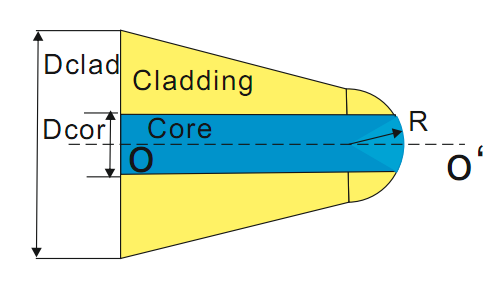
\includegraphics[width=0.4\textwidth]{bilder/lense_fiber_01}
\label{fig:lense_fiber_01}
}
\hfill
\subfigure[Tapered core TLF.]{
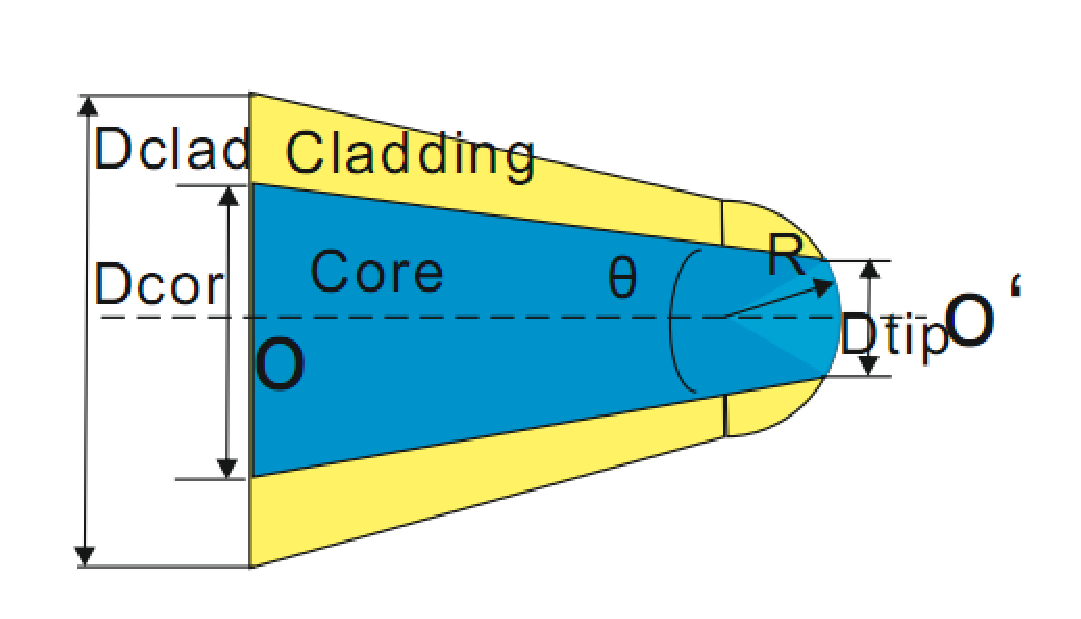
\includegraphics[width=0.4\textwidth]{bilder/lense_fiber_02}
\label{fig:lense_fiber_02}
}
\label{fig:two_TLF}
\caption{Two types of Tapered and Lensed Fibers}
\end{figure}

The Tapered Cladding TLF Fig.\ref{fig:lense_fiber_01} shows that its cladding diameter decreases along the axis and its core diameter is a constant. For the Tapered Core TLF Fig.\ref{fig:lense_fiber_02} its cladding diameter and core diameter both decrease along the axis. \cite{TLF_mode_transforming} develops method to estimate the performance of both type of TLF.  And results show that the performance of the first type of TLF agrees well with the estimation and that of the second type is unpredictable. 

Create two TLF models from each type and test the performances in CST MWS. The following Tab.\ref{tab:model_fiber_configuration} indicates the corresponding configurations.

\begin{table}
\begin{tabular}{ccc}
\hline
							&Tapered Cladding&Tapered Core\\
\hline
$R(\mu m)$ & $6$						 &$6$	\\
refractive indices(core)&$1.68$&$1.66$\\
refractive indices(cladding)&$1.68$&$1.66$\\
$D_{clad}(\mu m)$ &	$17$ &	$17$\\
$D_{core}(\mu m)$ & $10$ &	$17$\\
$D_{tip}(\mu m)$  & --   &	$10$\\
\hline
\end{tabular}
\caption{The Configurations of the TLF Models}
\label{tab:model_fiber_configuration}
\end{table}



\begin{figure}
\setlength{\abovecaptionskip}{0pt}% 
\flushleft
	\subfigure[sub1]{
	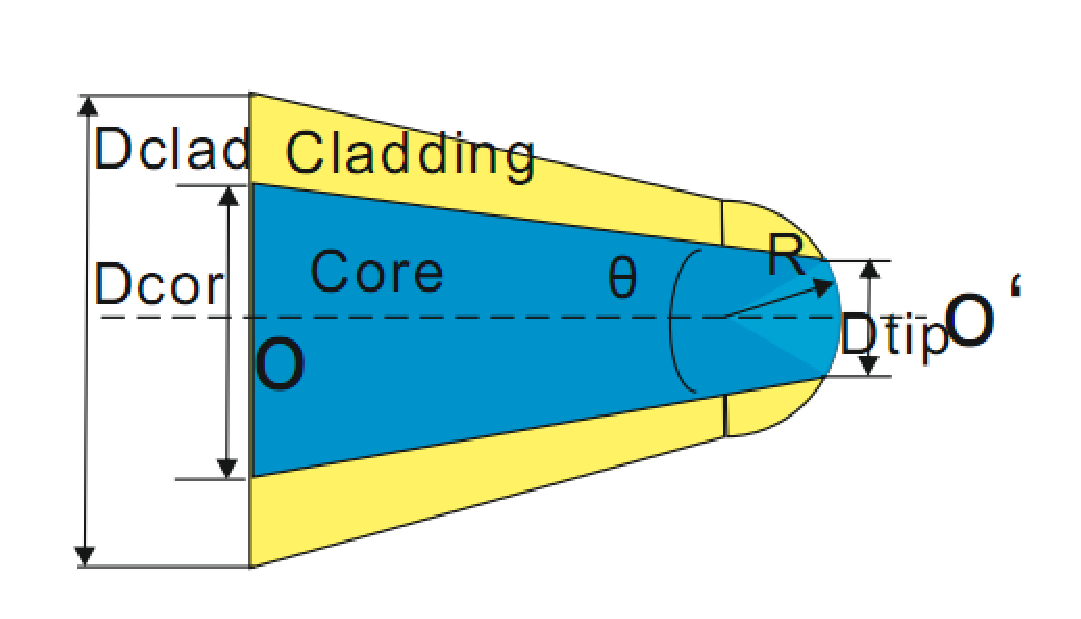
\includegraphics[width=0.23 \textwidth]{bilder/lense_fiber_02}
	\label{fig:subfigure1}%
	}

 	\subfigure[sub2]{
 	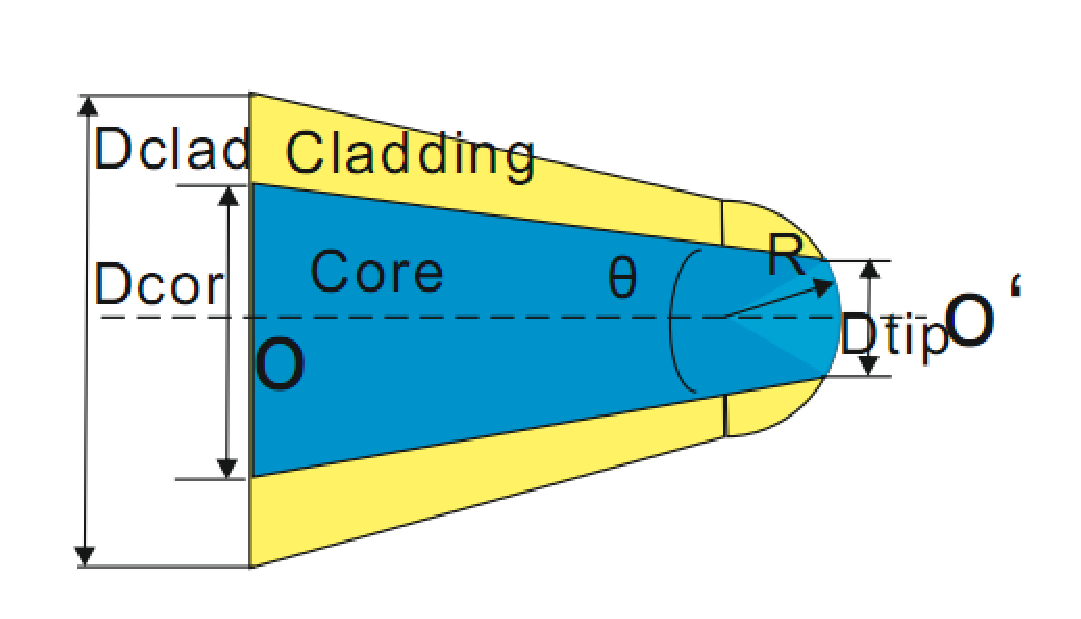
\includegraphics[width=0.23 \textwidth]{bilder/lense_fiber_02}
 	\label{fig:subfigure2}
 	}
 	 	\subfigure[sub2]{
 	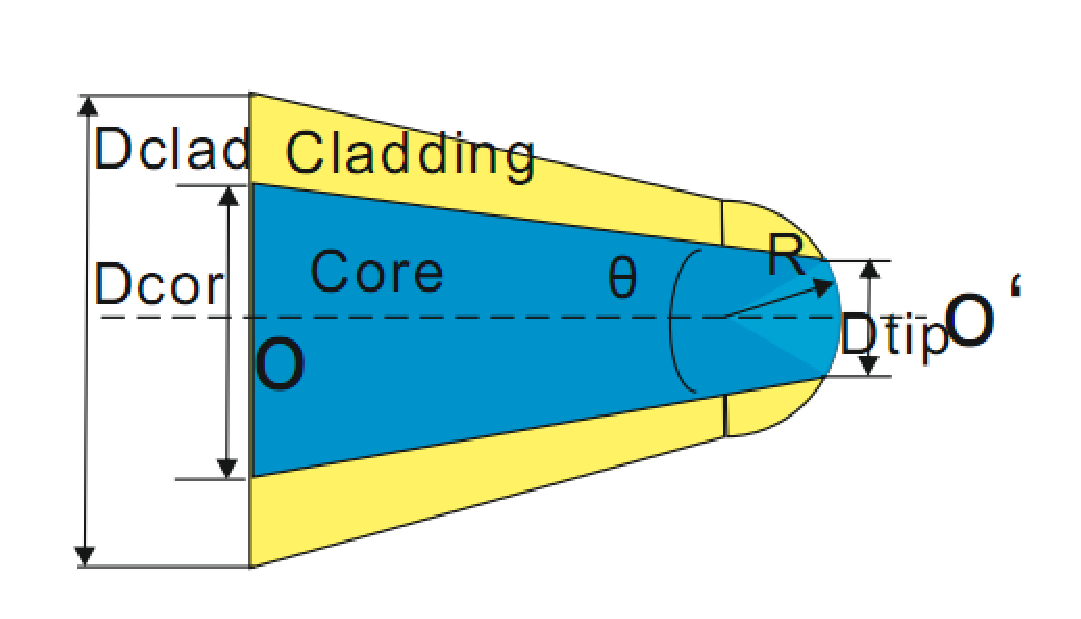
\includegraphics[width=0.23 \textwidth]{bilder/lense_fiber_02}
 	\label{fig:subfigure3}
 	}
 	 	\subfigure[sub2]{
 	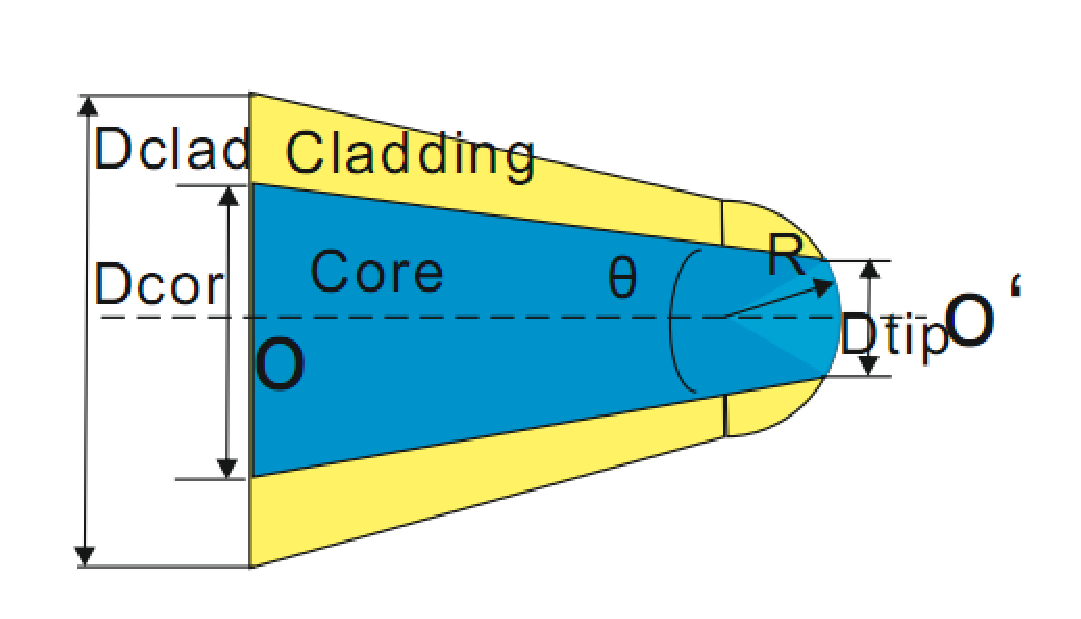
\includegraphics[width=0.23 \textwidth]{bilder/lense_fiber_02}
 	\label{fig:subfigure4}
 	}
 	 	\subfigure[sub2]{
 	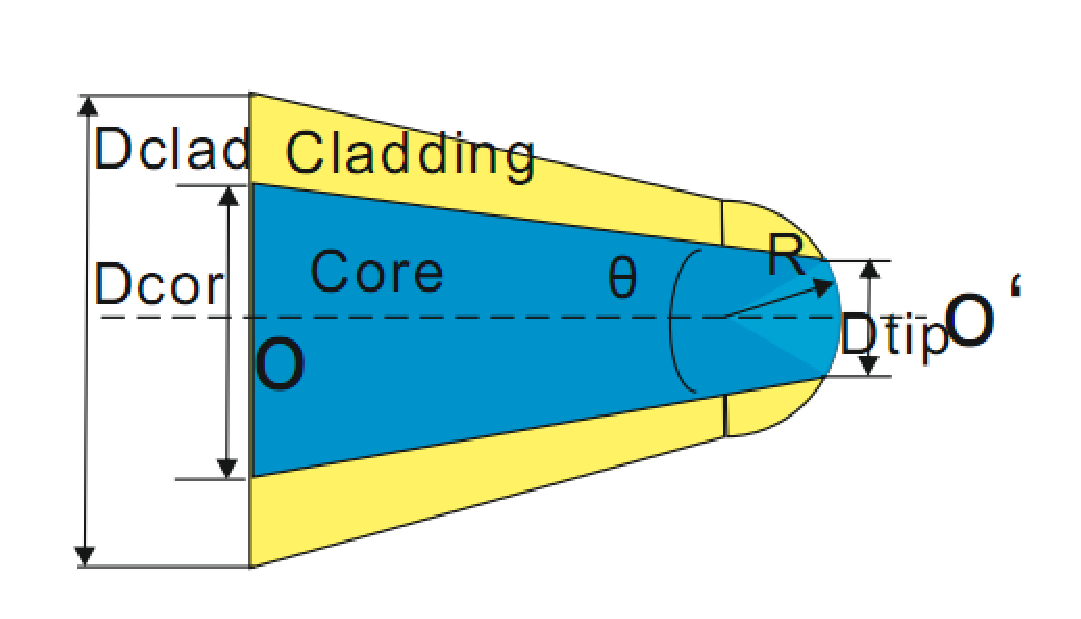
\includegraphics[width=0.23 \textwidth]{bilder/lense_fiber_02}
 	\label{fig:subfigure5}
 	}
\end{figure}

%2.20
The fowllowing is the E-Field demonstration in the xz-plane.
\begin{figure}
	\subfigure[E-Field demonstration of Tapered cladding TLF]{
		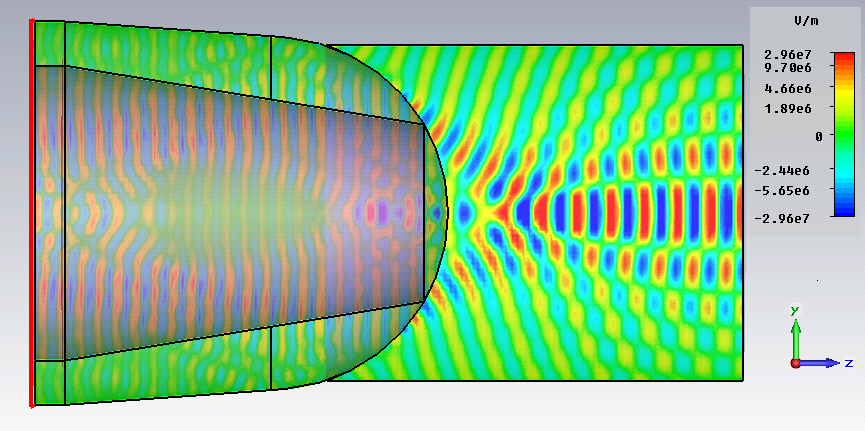
\includegraphics[width=0.4 \textwidth]{bilder/cst_lensed_fiber_efield}
 		\label{fig:Tapered_cladding_efield}
	}
	\subfigure[E-Field demonstration of Tapered core TLF]{
		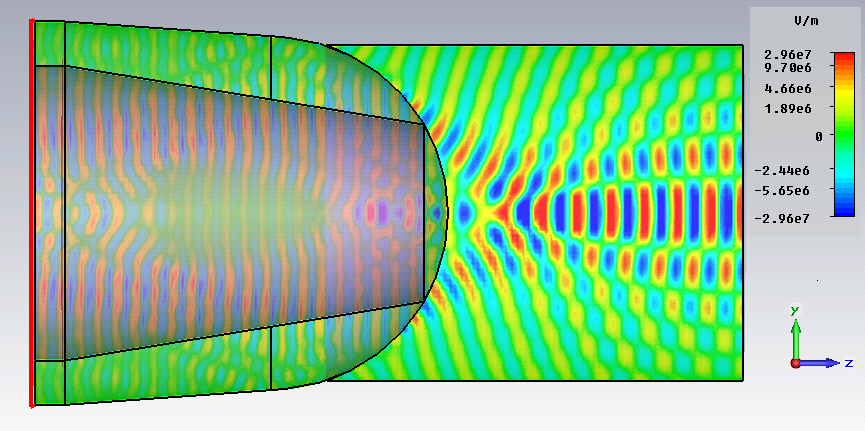
\includegraphics[width=0.4 \textwidth]{bilder/cst_lensed_fiber_efield}
 		\label{fig:Tapered_core_efield}	
	}
	\caption{E Field demonstration}
\end{figure}
As is in section lense theory introduced, the minimum spot located not exactly at the focal length. By using the location of PP and that of MP the MS can be estimated. The theoretical distance from lens end to PP is $xx \mu m$ and the distance from lens end to MP is  $xx \mu m$. Backword $3/4$ LAM form PP, the MS is founded at about $xx \mu m$far from lens end. Through The following figure is the theoretical beam propagation of the lense model.
Load the its beam propagation detail into \textbf{Matlab} workspace and check the beam power distribution in different distance. Fig.(\ref{}-\ref{}).%2D and 3D

\begin{figure}
\end{figure}
 
Draw Fig.\ref{}-\ref{} to illustrate the beam Spot size diameter along the longitude axis.

\begin{figure}
\caption{Curve of Spot size diameter}
\end{figure}
From Fig.\ref{tapered cladding} that the minimum spot size locate at $xxx \mu m$ from lense end and spot size equal about $1.7 \mu m$. While in Fig.\ref{tapered core} that the minimum spot size is found at  $xxx \mu m$ from lense end and spot size equal about $1.5 \mu m$. Thus it is concluded that tapered core TLF has a bit higher focal performance. By rechecking the properties in Tab.\ref{} both TLF model are acceptable for the following development. In this article the Tapered core TLF will be used for further simulations. 
